
\documentclass[12pt, a4, twoside]{report}

% DEFAULT PACKAGE SETUP
\usepackage{setspace,graphicx,epstopdf,amsmath,amsfonts,amssymb,amsthm}
\usepackage{marginnote,datetime,enumitem,rotating, fancyvrb}
\usepackage{hyperref, float}
\usepackage{verbatim}
\usepackage{booktabs}
\usepackage{subfigure}
\usepackage[longnamesfirst]{natbib}
\usdate

%For referencing theorems and lemmas
\usepackage{cleveref}% http://ctan.org/pkg/cleveref
\usepackage{arydshln}

% Deal with multiple bibliographies
\usepackage{emptypage}
\usepackage{multibib}
\newcites{Somm}{References}
\newcites{Intro}{References}
\newcites{One}{References}
\newcites{Two}{References}
\newcites{Three}{References}

% Number paragraphs and subparagraphs and include them in TOC
\setcounter{tocdepth}{2}

% JFE-specific includes:

\usepackage{indentfirst} % Indent first sentence of a new section.
\usepackage{jfe}          % JFE-specific formatting of sections, etc.

% Set margins
\usepackage[margin=1in]{geometry}
\usepackage{accents}

% Theorem titles
\newtheorem{theorem}{Theorem}[section]
\newtheorem{claim}{Claim}
\newtheorem{assumption}{Assumption}[section]
\newtheorem{proposition}{Proposition}
\newtheorem{conjecture}{Conjecture}
\newtheorem{lemma}{Lemma} %[section]
\newtheorem{corollary}{Corollary}
\newtheorem{condition}{Condition}
\newtheorem{definition}{Definition}

% For cref
\crefname{lemma}{Lemma}{Lemmas}
\crefname{claim}{Claim}{Claims}
\crefname{proposition}{Proposition}{Propostions}
\crefname{figure}{Figure}{Figures}
\crefname{table}{Table}{Tables}
\crefname{equation}{Eq.}{Eqs.}
\crefname{algocf}{Algorithm}{Algorithms}
\crefname{appendix}{Appendix}{Appendices}
\crefname{appsec}{Appendix}{Appendices}


% needed?
%\newcommand\subfigsize{0.5\textwidth}
%\newcommand{\omegvec}{\bm{\omega}}

% needed?
%\newcommand\munderbar[1]{%
%	\underaccent{\bar}{#1}}

%\newcolumntype{d}[1]{D..{#1}} % for alignment of numbers on decimal marker

% For dealing with multiple appendices
\makeatletter
\newcounter{savesection}
\newcounter{apdxsection}
\renewcommand\appendix{\par
	\setcounter{savesection}{\value{section}}%
	\setcounter{section}{\value{apdxsection}}%
	\setcounter{subsection}{0}%
	\gdef\thesection{\@Alph\c@section}}
\newcommand\unappendix{\par
	%\setcounter{apdxsection}{\value{section}}%
	\setcounter{apdxsection}{0}%
	\setcounter{section}{\value{savesection}}%
	\setcounter{subsection}{0}%
	\gdef\thesection{\@arabic\c@section}}
\makeatother

% For dealing with pagecount around abstracts
\makeatletter
\newcounter{stored_pagecount}
\makeatother

% Reset counters at starts of chapters
\makeatletter
\@addtoreset{theorem}{chapter}
\@addtoreset{proposition}{chapter}
\makeatother

% Redefine chapter heading to reduce whitespace
\makeatletter
\renewcommand*\@makechapterhead[1]{%
	%\vspace*{50\p@}%
	{\parindent \z@ \raggedright \normalfont
		\ifnum \c@secnumdepth >\m@ne
		\huge\bfseries \@chapapp\space \thechapter
		\par\nobreak
		\vskip 20\p@
		\fi
		\interlinepenalty\@M
		\Huge \bfseries #1\par\nobreak
		%\vskip 40\p@
	}}
\makeatother

% needed?
% \setlist{noitemsep}  % Reduce space between list items (itemize, enumerate, etc.)

% needed?
%\makeatletter
%\renewcommand*\env@matrix[1][*\c@MaxMatrixCols c]{%
%	\hskip -\arraycolsep
%	\let\@ifnextchar\new@ifnextchar
%	\array{#1}}
%\makeatother

\begin{document}

	\setlist{noitemsep}  % Reduce space between list items (itemize, enumerate, etc.)

	\singlespacing

    \begin{titlepage}
\begin{center}
    \vspace*{1cm}

    \Large
    \textbf{Institut d'\'etudes politiques de Paris}\\
    \textbf{\'ECOLE DOCTORALE DE SCIENCES PO}\\
    \textbf{Programme doctoral en \'economie}\\
    \textbf{D\'epartement d'\'Economie}\\
    \textbf{Doctorat en sciences \'economiques}\\

    \vspace{1.5cm}
    \Huge
    An Amazing Thesis

    %\vspace{0.5cm}
    %\Huge
    %Sous-titre

    \vspace{0.5cm}
    \Large
    Joey "The Smartest" Macmillan

    \vfill

    Thesis supervised by\\
     Smartest Ever, Professor of Smart Stuff, IEP de Paris\\
    Defended on 1 July, 2019

    \vspace{0.8cm}


\large

\noindent Jury:\\
\hspace{-0.0cm}Mrs. Sheryl CROW, Professeur de confusion, Another University\\
\hspace{-0.0cm}Mrs. Sheryl CROW, Professeur de confusion, Another University\\
\hspace{-0.0cm}Mrs. Sheryl CROW, Professeur de confusion, Another University\\
\hspace{-0.0cm}Mrs. Sheryl CROW, Professeur de confusion, Another University\\
\end{center}
\end{titlepage}

\setcounter{page}{2}


    \cleardoublepage
	
    \begin{titlepage}
\begin{center}
    \vspace*{1cm}

    \Large
    \textbf{Institut d'\'etudes politiques de Paris}\\
    \textbf{\'ECOLE DOCTORALE DE SCIENCES PO}\\
    \textbf{Programme doctoral en \'economie}\\
    \textbf{D\'epartement d'\'Economie}\\
    \textbf{Doctorat en sciences \'economiques}\\

    \vspace{1.5cm}
    \Huge
    An Amazing Thesis

    %\vspace{0.5cm}
    %\Huge
    %Sous-titre

    \vspace{0.5cm}
    \Large
    Joey "The Smartest" Macmillan

    \vfill

    Th\`ese dirig\'ee par\\
     Smartest Ever, Professor of Smart Stuff, IEP de Paris\\
    Soutenue le 1 juillet, 2019

    \vspace{0.8cm}


\large

\centering
\noindent Jury:\\
\hspace{-0.0cm}Mrs. Sheryl CROW, Professeur de confusion, Another University\\
\hspace{-0.0cm}Mrs. Sheryl CROW, Professeur de confusion, Another University\\
\hspace{-0.0cm}Mrs. Sheryl CROW, Professeur de confusion, Another University\\
\hspace{-0.0cm}Mrs. Sheryl CROW, Professeur de confusion, Another University\\
\end{center}
\end{titlepage}

\setcounter{page}{2}


    \cleardoublepage

	
\raggedbottom

\onehalfspacing
\setcounter{footnote}{0}
\renewcommand{\thefootnote}{\arabic{footnote}}


\chapter*{Acknowledgements}

Lorem ipsum dolor sit amet, consectetur adipiscing elit. Sed sollicitudin massa vel venenatis dictum. Aliquam erat volutpat. Phasellus accumsan eu felis at luctus. Integer neque elit, venenatis sed iaculis in, tincidunt nec augue. Aliquam erat volutpat. Nulla sodales tortor non justo tincidunt, non varius risus mollis. Aliquam est purus, cursus at nulla ac, sollicitudin placerat diam. Vestibulum ante ipsum primis in faucibus orci luctus et ultrices posuere cubilia Curae; Ut at leo eget metus scelerisque venenatis. Sed quis dui nisi. Morbi sodales, leo ac scelerisque malesuada, libero sem placerat ante, sit amet ullamcorper ligula nulla vestibulum tellus.

    % cleardoublepage ensures section begins on odd page
    \cleardoublepage
	\tableofcontents

    \cleardoublepage
	\listoffigures

    \cleardoublepage
	\listoftables

    % Ensure that appendix numbering properly initialized
	\unappendix

    \cleardoublepage
  \chapter*{Sommaire}
\addcontentsline{toc}{chapter}{Sommaire}

\raggedbottom

\onehalfspacing
\setcounter{footnote}{0}
\renewcommand{\thefootnote}{\arabic{footnote}}

Lorem \citeSomm{smith2019title} ipsum dolor sit amet, consectetur adipiscing elit. Sed sollicitudin massa vel venenatis dictum. Aliquam erat volutpat. Phasellus accumsan eu felis at luctus. Integer neque elit, venenatis sed iaculis in, tincidunt nec augue. Aliquam erat volutpat. Nulla sodales tortor non justo tincidunt, non varius risus mollis. Aliquam est purus, cursus at nulla ac, sollicitudin placerat diam. Vestibulum ante ipsum primis in faucibus orci luctus et ultrices posuere cubilia Curae; Ut at leo eget metus scelerisque venenatis. Sed quis dui nisi. Morbi sodales, leo ac scelerisque malesuada, libero sem placerat ante, sit amet ullamcorper ligula nulla vestibulum tellus.



\bibliographystyleSomm{apalike}
\bibliographySomm{/home/tmabbot/MEGA/Writing/mybib}


    \cleardoublepage
	\chapter*{Introduction}
\addcontentsline{toc}{chapter}{Introduction}

\raggedbottom

\onehalfspacing
\setcounter{footnote}{0}
\renewcommand{\thefootnote}{\arabic{footnote}}

Lorem ipsum dolor sit amet, consectetur adipiscing elit. Sed sollicitudin massa vel venenatis dictum. Aliquam erat volutpat. Phasellus accumsan eu felis at luctus. Integer neque elit, \citeIntro{smith2019title} venenatis sed iaculis in, tincidunt nec augue. Aliquam erat volutpat. Nulla sodales tortor non justo tincidunt, non varius risus mollis. Aliquam est purus, cursus at nulla ac, sollicitudin placerat diam. Vestibulum ante ipsum primis in faucibus orci luctus et ultrices posuere cubilia Curae; Ut \citeIntro{smith2019title}
at leo eget metus scelerisque venenatis. Sed quis dui nisi. Morbi sodales, leo ac scelerisque malesuada, libero sem placerat ante, \citeIntro{smith2019title} sit amet ullamcorper ligula nulla vestibulum tellus.


\section*{Chapter 1: A Great Chapter}

Lorem ipsum dolor sit amet, consectetur adipiscing elit. Sed sollicitudin massa vel venenatis dictum. Aliquam erat volutpat. Phasellus accumsan eu felis at luctus. Integer neque elit, \citeIntro{smith2019title} venenatis sed iaculis in, tincidunt nec augue. Aliquam erat volutpat. Nulla sodales tortor non justo tincidunt, non varius risus mollis. Aliquam est purus, cursus at nulla ac, sollicitudin placerat diam. Vestibulum ante ipsum primis in faucibus orci luctus et ultrices posuere cubilia Curae; Ut \citeIntro{smith2019title}
at leo eget metus scelerisque venenatis. Sed quis dui nisi. Morbi sodales, leo ac scelerisque malesuada, libero sem placerat ante, \citeIntro{smith2019title} sit amet ullamcorper ligula nulla vestibulum tellus.

\section*{Chapter 2: A Great Chapter}

Lorem ipsum dolor sit amet, consectetur adipiscing elit. Sed sollicitudin massa vel venenatis dictum. Aliquam erat volutpat. Phasellus accumsan eu felis at luctus. Integer neque elit, \citeIntro{smith2019title} venenatis sed iaculis in, tincidunt nec augue. Aliquam erat volutpat. Nulla sodales tortor non justo tincidunt, non varius risus mollis. Aliquam est purus, cursus at nulla ac, sollicitudin placerat diam. Vestibulum ante ipsum primis in faucibus orci luctus et ultrices posuere cubilia Curae; Ut \citeIntro{smith2019title}
at leo eget metus scelerisque venenatis. Sed quis dui nisi. Morbi sodales, leo ac scelerisque malesuada, libero sem placerat ante, \citeIntro{smith2019title} sit amet ullamcorper ligula nulla vestibulum tellus.

\section*{Chapter 3: A Great Chapter}

Lorem ipsum dolor sit amet, consectetur adipiscing elit. Sed sollicitudin massa vel venenatis dictum. Aliquam erat volutpat. Phasellus accumsan eu felis at luctus. Integer neque elit, \citeIntro{smith2019title} venenatis sed iaculis in, tincidunt nec augue. Aliquam erat volutpat. Nulla sodales tortor non justo tincidunt, non varius risus mollis. Aliquam est purus, cursus at nulla ac, sollicitudin placerat diam. Vestibulum ante ipsum primis in faucibus orci luctus et ultrices posuere cubilia Curae; Ut \citeIntro{smith2019title}
at leo eget metus scelerisque venenatis. Sed quis dui nisi. Morbi sodales, leo ac scelerisque malesuada, libero sem placerat ante, \citeIntro{smith2019title} sit amet ullamcorper ligula nulla vestibulum tellus.

\bibliographystyleIntro{apalike}
\bibliographyIntro{mybib}


    \cleardoublepage
	
% Fix alignment and ensure title, abstract, and text all on same page
\begin{flushleft}
\begin{minipage}{\textwidth}

\chapter{A Great Chapter}\label{chapter1}

% Store page number since abstract kills it
\setcounter{stored_pagecount}{\value{page}}
\begin{abstract}
	\thispagestyle{plain}
Lorem ipsum dolor sit amet, consectetur adipiscing elit. Sed sollicitudin massa vel venenatis dictum. Aliquam erat volutpat. Phasellus accumsan eu felis at luctus. Integer neque elit, venenatis sed iaculis in, tincidunt nec augue. Aliquam erat volutpat. Nulla sodales tortor non justo tincidunt, non varius risus mollis. Aliquam est purus, cursus at nulla ac, sollicitudin placerat diam. Vestibulum ante ipsum primis in faucibus orci luctus et ultrices posuere cubilia Curae; Ut at leo eget metus scelerisque venenatis. Sed quis dui nisi. Morbi sodales, leo ac scelerisque malesuada, libero sem placerat ante, sit amet ullamcorper ligula nulla vestibulum tellus.
\end{abstract}

% Reset since abstract kills it
\setcounter{page}{\value{stored_pagecount}}

\end{minipage}
\end{flushleft}

\onehalfspacing
\setcounter{footnote}{0}
\renewcommand{\thefootnote}{\arabic{footnote}}
%\setcounter{page}{1}

\section*{Introduction}

Lorem ipsum dolor sit amet, consectetur adipiscing elit. Sed sollicitudin massa vel venenatis dictum. Aliquam erat volutpat. Phasellus accumsan eu felis at luctus. Integer neque elit, \citeOne{smith2019title} venenatis sed iaculis in, tincidunt nec augue. Aliquam erat volutpat. Nulla sodales tortor non justo tincidunt, non varius risus mollis. Aliquam est purus, cursus at nulla ac, sollicitudin placerat diam. Vestibulum ante ipsum primis in faucibus orci luctus et ultrices posuere cubilia Curae; Ut \citeOne{smith2019title}
at leo eget metus scelerisque venenatis. Sed quis dui nisi. Morbi sodales, leo ac scelerisque malesuada, libero sem placerat ante, \citeOne{smith2019title} sit amet ullamcorper ligula nulla vestibulum tellus.

Lorem \Cref{sec:One} ipsum dolor sit amet, consectetur adipiscing elit. Sed sollicitudin massa vel venenatis dictum. Aliquam erat volutpat. Phasellus accumsan eu felis at luctus. Integer neque elit, venenatis sed iaculis in, tincidunt nec augue. Aliquam erat volutpat. Nulla sodales tortor non justo tincidunt, non varius risus mollis. Aliquam est purus, cursus at nulla ac, sollicitudin placerat diam. Vestibulum ante ipsum primis in faucibus orci luctus et ultrices posuere cubilia Curae; Ut at leo eget metus scelerisque venenatis. Sed quis dui nisi. Morbi sodales, leo ac scelerisque malesuada, libero sem placerat ante, sit amet ullamcorper ligula nulla vestibulum tellus.


\section{A Section} \label{sec:One}
Lorem ipsum dolor sit amet, consectetur adipiscing elit. Sed sollicitudin massa vel venenatis dictum. Aliquam erat volutpat. Phasellus accumsan eu felis at luctus. Integer neque elit, venenatis sed iaculis in, tincidunt nec augue. Aliquam erat volutpat. Nulla sodales tortor non justo tincidunt, non varius risus mollis. Aliquam est purus, cursus at nulla ac, sollicitudin placerat diam. Vestibulum ante ipsum primis in faucibus orci luctus et ultrices posuere cubilia Curae; Ut at leo eget metus scelerisque venenatis. Sed quis dui nisi. Morbi sodales, leo ac scelerisque malesuada, libero sem placerat ante, sit amet ullamcorper ligula nulla vestibulum tellus.

\begin{proposition}\label{prop:important}
 	Bla bla bla
	\begin{align*}
		y=a + bx
	\end{align*}
 	which admits a unique solution in $x$.
\end{proposition}
\noindent Lorem ipsum \cref{prop:important} dolor sit amet, consectetur adipiscing elit. Sed sollicitudin massa vel venenatis dictum.


\subsection{A Subsection}
Lorem ipsum dolor sit amet, consectetur adipiscing elit. Sed sollicitudin massa vel venenatis dictum. Aliquam erat volutpat. Phasellus accumsan eu felis at luctus. Integer neque elit, venenatis sed iaculis in, tincidunt nec augue. Aliquam erat volutpat. Nulla sodales tortor non justo tincidunt, non varius risus mollis. Aliquam est purus, cursus at nulla ac, sollicitudin placerat diam. Vestibulum ante ipsum primis in faucibus orci luctus et ultrices posuere cubilia Curae; Ut at leo eget metus scelerisque venenatis. Sed quis dui nisi. Morbi sodales, leo ac scelerisque malesuada, libero sem placerat ante, sit amet ullamcorper ligula nulla vestibulum tellus.

\begin{figure}[!h]
	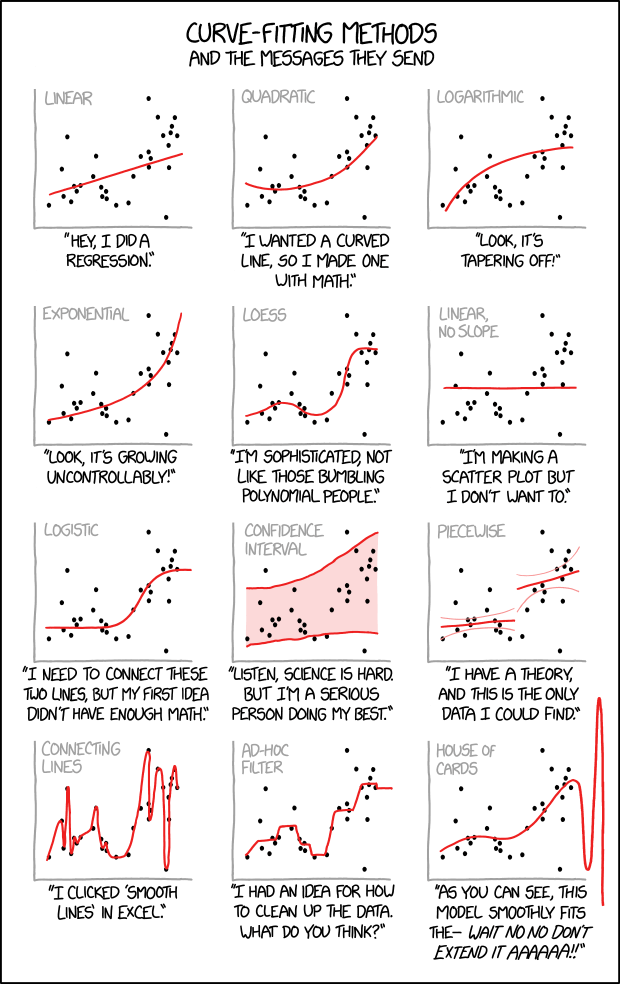
\includegraphics[width=0.8\textwidth]{plots/curve_fitting}
	\centering
	\caption{Important graphs for my research.}
	\centering
	\label{fig:curve_fitting}
\end{figure}

Lorem ipsum dolor sit amet, consectetur adipiscing elit. Sed sollicitudin massa vel venenatis dictum. Aliquam erat volutpat. Phasellus accumsan eu felis at luctus. Integer neque elit, venenatis sed iaculis \cref{fig:curve_fitting} in, tincidunt nec augue. Aliquam erat volutpat. Nulla sodales tortor non justo tincidunt, non varius risus mollis. Aliquam est purus, cursus at nulla ac, sollicitudin placerat diam. Vestibulum ante ipsum primis in faucibus orci luctus et ultrices posuere cubilia Curae; Ut at leo eget metus scelerisque venenatis. Sed quis dui nisi. Morbi sodales, leo ac scelerisque malesuada, libero sem placerat ante, sit amet ullamcorper ligula nulla vestibulum tellus.

\begin{figure}[!h]
	\hspace{-5pt}
	\subfigure[Scheduling]{
		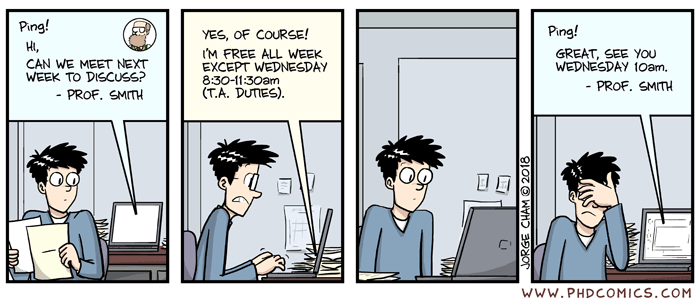
\includegraphics[width=0.5\textwidth]{plots/advisor1}
		%\centering
		%\caption{}
		%\centering
		\label{fig:advisor1}
	}\hspace{-10pt}
	\subfigure[Imposter Syndrome]{
		
\includegraphics[width=0.5\textwidth]{plots/advisor2}
		\centering
		%\caption{}
		%\centering
		\label{fig:advisor2}
	}
	\caption{\cref{fig:advisor1} is funny, but so is \cref{fig:advisor2}.}
	\label{fig:advisors}
\end{figure}

Lorem ipsum dolor sit amet, consectetur adipiscing elit. Sed sollicitudin massa vel venenatis dictum. Aliquam erat volutpat. Phasellus accumsan eu felis at luctus. Integer neque elit, venenatis sed iaculis \cref{fig:advisor1,fig:advisor2} in, tincidunt nec augue. Aliquam erat volutpat. Nulla sodales tortor non justo tincidunt, non varius risus mollis. Aliquam est purus, cursus at nulla ac,\cref{fig:advisors} sollicitudin placerat diam. Vestibulum ante ipsum primis in faucibus orci luctus et ultrices posuere cubilia Curae; Ut at leo eget metus scelerisque venenatis. Sed quis dui nisi. Morbi sodales, leo ac scelerisque malesuada, libero sem placerat ante, sit amet ullamcorper ligula nulla vestibulum tellus.

\section{Conclusion} \label{sec:conc}
Lorem ipsum dolor sit amet, consectetur adipiscing elit. Sed sollicitudin massa vel venenatis dictum. Aliquam erat volutpat. Phasellus accumsan eu felis at luctus. Integer neque elit, venenatis sed iaculis in, tincidunt nec augue. Aliquam erat volutpat. Nulla sodales tortor non justo tincidunt, non varius risus mollis. Aliquam est purus, cursus at nulla ac, sollicitudin placerat diam. Vestibulum ante ipsum primis in faucibus orci luctus et ultrices posuere cubilia Curae; Ut at leo eget metus scelerisque venenatis. Sed quis dui nisi. Morbi sodales, leo ac scelerisque malesuada, libero sem placerat ante, sit amet ullamcorper ligula nulla vestibulum tellus.



\bibliographystyleOne{apalike}
\bibliographyOne{mybib}
\clearpage

\appendix

% Start naming sections appendix
\crefalias{section}{appendix}

\section{Proofs}

\begin{proof}[Proof of \cref{prop:important}]
 	Bla bla bla
 	\begin{align*}
 	y=a + bx
 	\end{align*}
 	which admits a unique solution in $x$.
\end{proof}

\section{An Important Thing That Didn't Make The Cut}\label[appendix]{sec:appendix_A}
Lorem ipsum dolor sit amet, consectetur adipiscing elit. Sed sollicitudin massa vel venenatis dictum. Aliquam erat volutpat. Phasellus accumsan eu felis at luctus. Integer neque elit, venenatis sed iaculis in, tincidunt nec augue. Aliquam erat volutpat. Nulla sodales tortor non justo tincidunt, non varius risus mollis. Aliquam est purus, cursus at nulla ac, sollicitudin placerat diam. Vestibulum ante ipsum primis in faucibus orci luctus et ultrices posuere cubilia Curae; Ut at leo eget metus scelerisque venenatis. Sed quis dui nisi. Morbi sodales, leo ac scelerisque malesuada, libero sem placerat ante, sit amet ullamcorper ligula nulla vestibulum tellus.


% Stop naming sections appendix
\unappendix
\crefalias{section}{section}


    \cleardoublepage
	
% Fix alignment and ensure title, abstract, and text all on same page
\begin{flushleft}
	\begin{minipage}{\textwidth}
		
		\chapter{A Great Chapter}\label{chapter2}
		
		% Store page number since abstract kills it
		\setcounter{stored_pagecount}{\value{page}}
		\begin{abstract}
			\thispagestyle{plain}
			Lorem ipsum dolor sit amet, consectetur adipiscing elit. Sed sollicitudin massa vel venenatis dictum. Aliquam erat volutpat. Phasellus accumsan eu felis at luctus. Integer neque elit, venenatis sed iaculis in, tincidunt nec augue. Aliquam erat volutpat. Nulla sodales tortor non justo tincidunt, non varius risus mollis. Aliquam est purus, cursus at nulla ac, sollicitudin placerat diam. Vestibulum ante ipsum primis in faucibus orci luctus et ultrices posuere cubilia Curae; Ut at leo eget metus scelerisque venenatis. Sed quis dui nisi. Morbi sodales, leo ac scelerisque malesuada, libero sem placerat ante, sit amet ullamcorper ligula nulla vestibulum tellus.
		\end{abstract}
		
		% Reset since abstract kills it
		\setcounter{page}{\value{stored_pagecount}}
		
	\end{minipage}
\end{flushleft}

\onehalfspacing
\setcounter{footnote}{0}
\renewcommand{\thefootnote}{\arabic{footnote}}
%\setcounter{page}{1}

\section*{Introduction}

Lorem ipsum dolor sit amet, consectetur adipiscing elit. Sed sollicitudin massa vel venenatis dictum. Aliquam erat volutpat. Phasellus accumsan eu felis at luctus. Integer neque elit, \citeTwo{smith2019title2} venenatis sed iaculis in, tincidunt nec augue. Aliquam erat volutpat. Nulla sodales tortor non justo tincidunt, non varius risus mollis. Aliquam est purus, cursus at nulla ac, sollicitudin placerat diam. Vestibulum ante ipsum primis in faucibus orci luctus et ultrices posuere cubilia Curae; Ut \citeTwo{smith2019title2}
at leo eget metus scelerisque venenatis. Sed quis dui nisi. Morbi sodales, leo ac scelerisque malesuada, libero sem placerat ante, \citeTwo{smith2019title2} sit amet ullamcorper ligula nulla vestibulum tellus.

Lorem \Cref{sec:One} ipsum dolor sit amet, consectetur adipiscing elit. Sed sollicitudin massa vel venenatis dictum. Aliquam erat volutpat. Phasellus accumsan eu felis at luctus. Integer neque elit, venenatis sed iaculis in, tincidunt nec augue. Aliquam erat volutpat. Nulla sodales tortor non justo tincidunt, non varius risus mollis. Aliquam est purus, cursus at nulla ac, sollicitudin placerat diam. Vestibulum ante ipsum primis in faucibus orci luctus et ultrices posuere cubilia Curae; Ut at leo eget metus scelerisque venenatis. Sed quis dui nisi. Morbi sodales, leo ac scelerisque malesuada, libero sem placerat ante, sit amet ullamcorper ligula nulla vestibulum tellus.


\section{A Section} \label{sec:One}
Lorem ipsum dolor sit amet, consectetur adipiscing elit. Sed sollicitudin massa vel venenatis dictum. Aliquam erat volutpat. Phasellus accumsan eu felis at luctus. Integer neque elit, venenatis sed iaculis in, tincidunt nec augue. Aliquam erat volutpat. Nulla sodales tortor non justo tincidunt, non varius risus mollis. Aliquam est purus, cursus at nulla ac, sollicitudin placerat diam. Vestibulum ante ipsum primis in faucibus orci luctus et ultrices posuere cubilia Curae; Ut at leo eget metus scelerisque venenatis. Sed quis dui nisi. Morbi sodales, leo ac scelerisque malesuada, libero sem placerat ante, sit amet ullamcorper ligula nulla vestibulum tellus.

\begin{proposition}\label{prop:important}
	Bla bla bla
	\begin{align*}
	y=a + bx
	\end{align*}
	which admits a unique solution in $x$.
\end{proposition}
\noindent Lorem ipsum \cref{prop:important} dolor sit amet, consectetur adipiscing elit. Sed sollicitudin massa vel venenatis dictum.


\subsection{A Subsection}
Lorem ipsum dolor sit amet, consectetur adipiscing elit. Sed sollicitudin massa vel venenatis dictum. Aliquam erat volutpat. Phasellus accumsan eu felis at luctus. Integer neque elit, venenatis sed iaculis in, tincidunt nec augue. Aliquam erat volutpat. Nulla sodales tortor non justo tincidunt, non varius risus mollis. Aliquam est purus, cursus at nulla ac, sollicitudin placerat diam. Vestibulum ante ipsum primis in faucibus orci luctus et ultrices posuere cubilia Curae; Ut at leo eget metus scelerisque venenatis. Sed quis dui nisi. Morbi sodales, leo ac scelerisque malesuada, libero sem placerat ante, sit amet ullamcorper ligula nulla vestibulum tellus.

\begin{figure}[!h]
	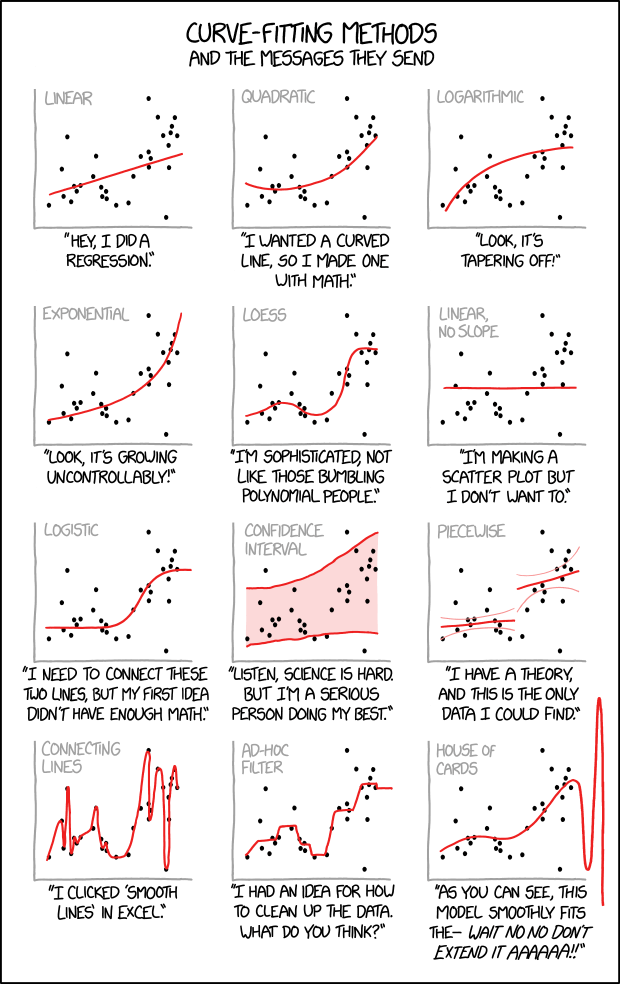
\includegraphics[width=0.8\textwidth]{plots/curve_fitting}
	\centering
	\caption{Important graphs for my research.}
	\centering
	\label{fig:curve_fitting}
\end{figure}

Lorem ipsum dolor sit amet, consectetur adipiscing elit. Sed sollicitudin massa vel venenatis dictum. Aliquam erat volutpat. Phasellus accumsan eu felis at luctus. Integer neque elit, venenatis sed iaculis \cref{fig:curve_fitting} in, tincidunt nec augue. Aliquam erat volutpat. Nulla sodales tortor non justo tincidunt, non varius risus mollis. Aliquam est purus, cursus at nulla ac, sollicitudin placerat diam. Vestibulum ante ipsum primis in faucibus orci luctus et ultrices posuere cubilia Curae; Ut at leo eget metus scelerisque venenatis. Sed quis dui nisi. Morbi sodales, leo ac scelerisque malesuada, libero sem placerat ante, sit amet ullamcorper ligula nulla vestibulum tellus.

\begin{figure}[!h]
	\hspace{-5pt}
	\subfigure[Scheduling]{
		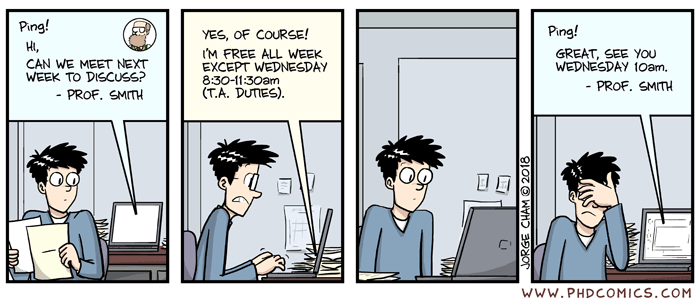
\includegraphics[width=0.5\textwidth]{plots/advisor1}
		%\centering
		%\caption{}
		%\centering
		\label{fig:advisor1}
	}\hspace{-10pt}
	\subfigure[Imposter Syndrome]{
		
\includegraphics[width=0.5\textwidth]{plots/advisor2}
		\centering
		%\caption{}
		%\centering
		\label{fig:advisor2}
	}
	\caption{\cref{fig:advisor1} is funny, but so is \cref{fig:advisor2}.}
	\label{fig:advisors}
\end{figure}

Lorem ipsum dolor sit amet, consectetur adipiscing elit. Sed sollicitudin massa vel venenatis dictum. Aliquam erat volutpat. Phasellus accumsan eu felis at luctus. Integer neque elit, venenatis sed iaculis \cref{fig:advisor1,fig:advisor2} in, tincidunt nec augue. Aliquam erat volutpat. Nulla sodales tortor non justo tincidunt, non varius risus mollis. Aliquam est purus, cursus at nulla ac,\cref{fig:advisors} sollicitudin placerat diam. Vestibulum ante ipsum primis in faucibus orci luctus et ultrices posuere cubilia Curae; Ut at leo eget metus scelerisque venenatis. Sed quis dui nisi. Morbi sodales, leo ac scelerisque malesuada, libero sem placerat ante, sit amet ullamcorper ligula nulla vestibulum tellus.

\section{Conclusion} \label{sec:conc}
Lorem ipsum dolor sit amet, consectetur adipiscing elit. Sed sollicitudin massa vel venenatis dictum. Aliquam erat volutpat. Phasellus accumsan eu felis at luctus. Integer neque elit, venenatis sed iaculis in, tincidunt nec augue. Aliquam erat volutpat. Nulla sodales tortor non justo tincidunt, non varius risus mollis. Aliquam est purus, cursus at nulla ac, sollicitudin placerat diam. Vestibulum ante ipsum primis in faucibus orci luctus et ultrices posuere cubilia Curae; Ut at leo eget metus scelerisque venenatis. Sed quis dui nisi. Morbi sodales, leo ac scelerisque malesuada, libero sem placerat ante, sit amet ullamcorper ligula nulla vestibulum tellus.



\bibliographystyleTwo{apalike}
\bibliographyTwo{mybib}
\clearpage

\appendix

% Start naming sections appendix
\crefalias{section}{appendix}

\section{Proofs}

\begin{proof}[Proof of \cref{prop:important}]
	Bla bla bla
	\begin{align*}
	y=a + bx
	\end{align*}
	which admits a unique solution in $x$.
\end{proof}

\section{An Important Thing That Didn't Make The Cut}\label[appendix]{sec:appendix_A}
Lorem ipsum dolor sit amet, consectetur adipiscing elit. Sed sollicitudin massa vel venenatis dictum. Aliquam erat volutpat. Phasellus accumsan eu felis at luctus. Integer neque elit, venenatis sed iaculis in, tincidunt nec augue. Aliquam erat volutpat. Nulla sodales tortor non justo tincidunt, non varius risus mollis. Aliquam est purus, cursus at nulla ac, sollicitudin placerat diam. Vestibulum ante ipsum primis in faucibus orci luctus et ultrices posuere cubilia Curae; Ut at leo eget metus scelerisque venenatis. Sed quis dui nisi. Morbi sodales, leo ac scelerisque malesuada, libero sem placerat ante, sit amet ullamcorper ligula nulla vestibulum tellus.


% Stop naming sections appendix
\unappendix
\crefalias{section}{section}




    \cleardoublepage
	
% Fix alignment and ensure title, abstract, and text all on same page
\begin{flushleft}
	\begin{minipage}{\textwidth}
		
		\chapter{A Great Chapter}\label{chapter1}
		
		% Store page number since abstract kills it
		\setcounter{stored_pagecount}{\value{page}}
		\begin{abstract}
			\thispagestyle{plain}
			Lorem ipsum dolor sit amet, consectetur adipiscing elit. Sed sollicitudin massa vel venenatis dictum. Aliquam erat volutpat. Phasellus accumsan eu felis at luctus. Integer neque elit, venenatis sed iaculis in, tincidunt nec augue. Aliquam erat volutpat. Nulla sodales tortor non justo tincidunt, non varius risus mollis. Aliquam est purus, cursus at nulla ac, sollicitudin placerat diam. Vestibulum ante ipsum primis in faucibus orci luctus et ultrices posuere cubilia Curae; Ut at leo eget metus scelerisque venenatis. Sed quis dui nisi. Morbi sodales, leo ac scelerisque malesuada, libero sem placerat ante, sit amet ullamcorper ligula nulla vestibulum tellus.
		\end{abstract}
		
		% Reset since abstract kills it
		\setcounter{page}{\value{stored_pagecount}}
		
	\end{minipage}
\end{flushleft}

\onehalfspacing
\setcounter{footnote}{0}
\renewcommand{\thefootnote}{\arabic{footnote}}
%\setcounter{page}{1}

\section*{Introduction}

Lorem ipsum dolor sit amet, consectetur adipiscing elit. Sed sollicitudin massa vel venenatis dictum. Aliquam erat volutpat. Phasellus accumsan eu felis at luctus. Integer neque elit, \citeThree{smith2019title} venenatis sed iaculis in, tincidunt nec augue. Aliquam erat volutpat. Nulla sodales tortor non justo tincidunt, non varius risus mollis. Aliquam est purus, cursus at nulla ac, sollicitudin placerat diam. Vestibulum ante ipsum primis in faucibus orci luctus et ultrices posuere cubilia Curae; Ut \citeThree{smith2019title}
at leo eget metus scelerisque venenatis. Sed quis dui nisi. Morbi sodales, leo ac scelerisque malesuada, libero sem placerat ante, \citeThree{smith2019title} sit amet ullamcorper ligula nulla vestibulum tellus.

Lorem \Cref{sec:One} ipsum dolor sit amet, consectetur adipiscing elit. Sed sollicitudin massa vel venenatis dictum. Aliquam erat volutpat. Phasellus accumsan eu felis at luctus. Integer neque elit, venenatis sed iaculis in, tincidunt nec augue. Aliquam erat volutpat. Nulla sodales tortor non justo tincidunt, non varius risus mollis. Aliquam est purus, cursus at nulla ac, sollicitudin placerat diam. Vestibulum ante ipsum primis in faucibus orci luctus et ultrices posuere cubilia Curae; Ut at leo eget metus scelerisque venenatis. Sed quis dui nisi. Morbi sodales, leo ac scelerisque malesuada, libero sem placerat ante, sit amet ullamcorper ligula nulla vestibulum tellus.


\section{A Section} \label{sec:One}
Lorem ipsum dolor sit amet, consectetur adipiscing elit. Sed sollicitudin massa vel venenatis dictum. Aliquam erat volutpat. Phasellus accumsan eu felis at luctus. Integer neque elit, venenatis sed iaculis in, tincidunt nec augue. Aliquam erat volutpat. Nulla sodales tortor non justo tincidunt, non varius risus mollis. Aliquam est purus, cursus at nulla ac, sollicitudin placerat diam. Vestibulum ante ipsum primis in faucibus orci luctus et ultrices posuere cubilia Curae; Ut at leo eget metus scelerisque venenatis. Sed quis dui nisi. Morbi sodales, leo ac scelerisque malesuada, libero sem placerat ante, sit amet ullamcorper ligula nulla vestibulum tellus.

\begin{proposition}\label{prop:important}
	Bla bla bla
	\begin{align*}
	y=a + bx
	\end{align*}
	which admits a unique solution in $x$.
\end{proposition}
\noindent Lorem ipsum \cref{prop:important} dolor sit amet, consectetur adipiscing elit. Sed sollicitudin massa vel venenatis dictum.


\subsection{A Subsection}
Lorem ipsum dolor sit amet, consectetur adipiscing elit. Sed sollicitudin massa vel venenatis dictum. Aliquam erat volutpat. Phasellus accumsan eu felis at luctus. Integer neque elit, venenatis sed iaculis in, tincidunt nec augue. Aliquam erat volutpat. Nulla sodales tortor non justo tincidunt, non varius risus mollis. Aliquam est purus, cursus at nulla ac, sollicitudin placerat diam. Vestibulum ante ipsum primis in faucibus orci luctus et ultrices posuere cubilia Curae; Ut at leo eget metus scelerisque venenatis. Sed quis dui nisi. Morbi sodales, leo ac scelerisque malesuada, libero sem placerat ante, sit amet ullamcorper ligula nulla vestibulum tellus.

\begin{figure}[!h]
	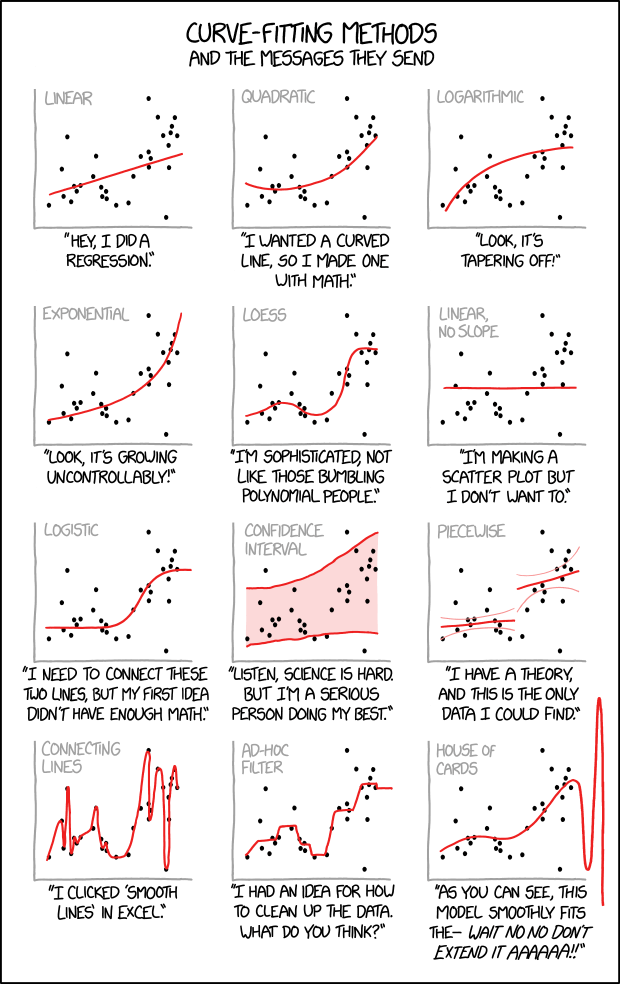
\includegraphics[width=0.8\textwidth]{plots/curve_fitting}
	\centering
	\caption{Important graphs for my research.}
	\centering
	\label{fig:curve_fitting}
\end{figure}

Lorem ipsum dolor sit amet, consectetur adipiscing elit. Sed sollicitudin massa vel venenatis dictum. Aliquam erat volutpat. Phasellus accumsan eu felis at luctus. Integer neque elit, venenatis sed iaculis \cref{curve_fitting} in, tincidunt nec augue. Aliquam erat volutpat. Nulla sodales tortor non justo tincidunt, non varius risus mollis. Aliquam est purus, cursus at nulla ac, sollicitudin placerat diam. Vestibulum ante ipsum primis in faucibus orci luctus et ultrices posuere cubilia Curae; Ut at leo eget metus scelerisque venenatis. Sed quis dui nisi. Morbi sodales, leo ac scelerisque malesuada, libero sem placerat ante, sit amet ullamcorper ligula nulla vestibulum tellus.

\begin{figure}[!h]
	\hspace{-5pt}
	\subfigure[Scheduling]{
		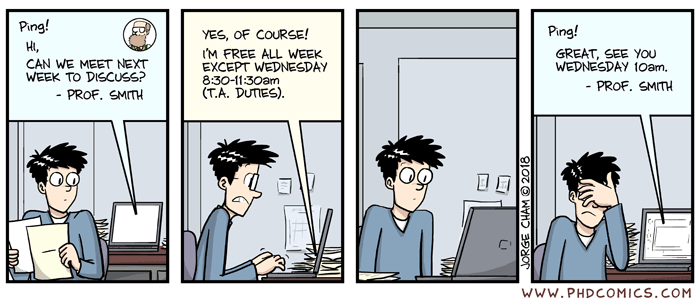
\includegraphics[width=0.5\textwidth]{plots/advisor1}
		%\centering
		%\caption{}
		%\centering
		\label{fig:advisor1}
	}\hspace{-10pt}
	\subfigure[Imposter Syndrome]{
		
\includegraphics[width=0.5\textwidth]{plots/advisor2}
		\centering
		%\caption{}
		%\centering
		\label{fig:advisor2}
	}
	\caption{\cref{fig:advisor1} is funny, but so is \cref{fig:advisor2}.}
	\label{fig:advisors}
\end{figure}

Lorem ipsum dolor sit amet, consectetur adipiscing elit. Sed sollicitudin massa vel venenatis dictum. Aliquam erat volutpat. Phasellus accumsan eu felis at luctus. Integer neque elit, venenatis sed iaculis \cref{fig:advisor1,fig:advisor2} in, tincidunt nec augue. Aliquam erat volutpat. Nulla sodales tortor non justo tincidunt, non varius risus mollis. Aliquam est purus, cursus at nulla ac,\cref{fig:advisors} sollicitudin placerat diam. Vestibulum ante ipsum primis in faucibus orci luctus et ultrices posuere cubilia Curae; Ut at leo eget metus scelerisque venenatis. Sed quis dui nisi. Morbi sodales, leo ac scelerisque malesuada, libero sem placerat ante, sit amet ullamcorper ligula nulla vestibulum tellus.

\section{Conclusion} \label{sec:conc}
Lorem ipsum dolor sit amet, consectetur adipiscing elit. Sed sollicitudin massa vel venenatis dictum. Aliquam erat volutpat. Phasellus accumsan eu felis at luctus. Integer neque elit, venenatis sed iaculis in, tincidunt nec augue. Aliquam erat volutpat. Nulla sodales tortor non justo tincidunt, non varius risus mollis. Aliquam est purus, cursus at nulla ac, sollicitudin placerat diam. Vestibulum ante ipsum primis in faucibus orci luctus et ultrices posuere cubilia Curae; Ut at leo eget metus scelerisque venenatis. Sed quis dui nisi. Morbi sodales, leo ac scelerisque malesuada, libero sem placerat ante, sit amet ullamcorper ligula nulla vestibulum tellus.



\bibliographystyleOne{apalike}
\bibliographyOne{mybib}
\clearpage

\appendix

% Start naming sections appendix
\crefalias{section}{appendix}

\section{Proofs}

\begin{proof}[Proof of \cref{prop:important}]
	Bla bla bla
	\begin{align*}
	y=a + bx
	\end{align*}
	which admits a unique solution in $x$.
\end{proof}

\section{An Important Thing That Didn't Make The Cut}\label[appendix]{sec:appendix_A}
Lorem ipsum dolor sit amet, consectetur adipiscing elit. Sed sollicitudin massa vel venenatis dictum. Aliquam erat volutpat. Phasellus accumsan eu felis at luctus. Integer neque elit, venenatis sed iaculis in, tincidunt nec augue. Aliquam erat volutpat. Nulla sodales tortor non justo tincidunt, non varius risus mollis. Aliquam est purus, cursus at nulla ac, sollicitudin placerat diam. Vestibulum ante ipsum primis in faucibus orci luctus et ultrices posuere cubilia Curae; Ut at leo eget metus scelerisque venenatis. Sed quis dui nisi. Morbi sodales, leo ac scelerisque malesuada, libero sem placerat ante, sit amet ullamcorper ligula nulla vestibulum tellus.


% Stop naming sections appendix
\unappendix
\crefalias{section}{section}



	
	  \cleardoublepage
  \chapter*{Conclusion}
\addcontentsline{toc}{chapter}{Conclusion}

\raggedbottom

\onehalfspacing
\setcounter{footnote}{0}
\renewcommand{\thefootnote}{\arabic{footnote}}

Lorem ipsum dolor sit amet, consectetur adipiscing elit. Sed sollicitudin massa vel venenatis dictum. Aliquam erat volutpat. Phasellus accumsan eu felis at luctus. Integer neque elit, venenatis sed iaculis in, tincidunt nec augue. Aliquam erat volutpat. Nulla sodales tortor non justo tincidunt, non varius risus mollis. Aliquam est purus, cursus at nulla ac, sollicitudin placerat diam. Vestibulum ante ipsum primis in faucibus orci luctus et ultrices posuere cubilia Curae; Ut at leo eget metus scelerisque venenatis. Sed quis dui nisi. Morbi sodales, leo ac scelerisque malesuada, libero sem placerat ante, sit amet ullamcorper ligula nulla vestibulum tellus.



\end{document}
